\documentclass[12pt,a4paper]{article}

\usepackage{fancyhdr}
\usepackage{graphicx}
\usepackage{placeins}
\usepackage{adjustbox}


\begin{document}

\pagestyle{fancy}
\fancyhf{}
\chead{Short summary report}

\begin{table}[t]
\centering
\caption {rnaQUAST metrics for assembled transcripts. In each row the best values are indicated with \textbf{bold}. For the transcript metrics (rows 2, 3) we highlighted the best \textbf{relative} values i.e. divided by the total number of transcripts in the corresponding assembly.}
\begin{adjustbox}{width=1\textwidth}
\small
\begin{tabular}{|l*{2}{|r}|}
\hline
\textbf{METRICS/TRANSCRIPTS}                            & \textbf{centroids}     \\ \hline\hline
\multicolumn{2}{l}{\bf BASIC TRANSCRIPTS METRICS}                                         \\ \hline
Transcripts                                             & 42092                  \\
Transcripts $>$ 500 bp                                  & \textbf{16521}         \\
Transcripts $>$ 1000 bp                                 & \textbf{8357}          \\ \hline
\end{tabular}
\end{adjustbox}
\end{table}

\FloatBarrier
\clearpage
\lfoot{generated by rnaQUAST}

\begin{figure}[t]
\centering
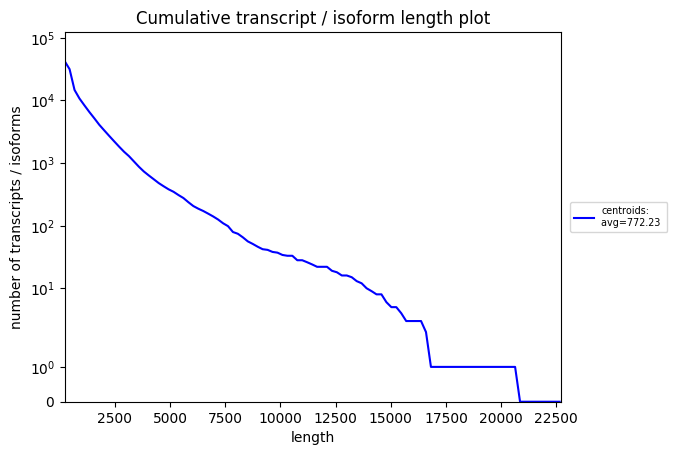
\includegraphics[width = \linewidth]{/labs/Knutie/BarretoNahomFrogs/modifiedanalysis/06_RNAQuast/transdecoderassembly/results/centroids_output/transcript_length.png}
\caption{Plot showing cumulative transcript length distribution. Each point represents the number of transcripts in the assembly with the corresponding length or longer; black dashed line corresponds to the database isoforms; the plot is given in logarithmic scale.}
\end{figure}
\FloatBarrier
\clearpage


\end{document}
